\section{Results}
\textit{- Present your \textbf{findings} in a logical and coherent manner.}

\begin{itemize}
    \item Environmental context
    
\begin{figure}
    \centering
    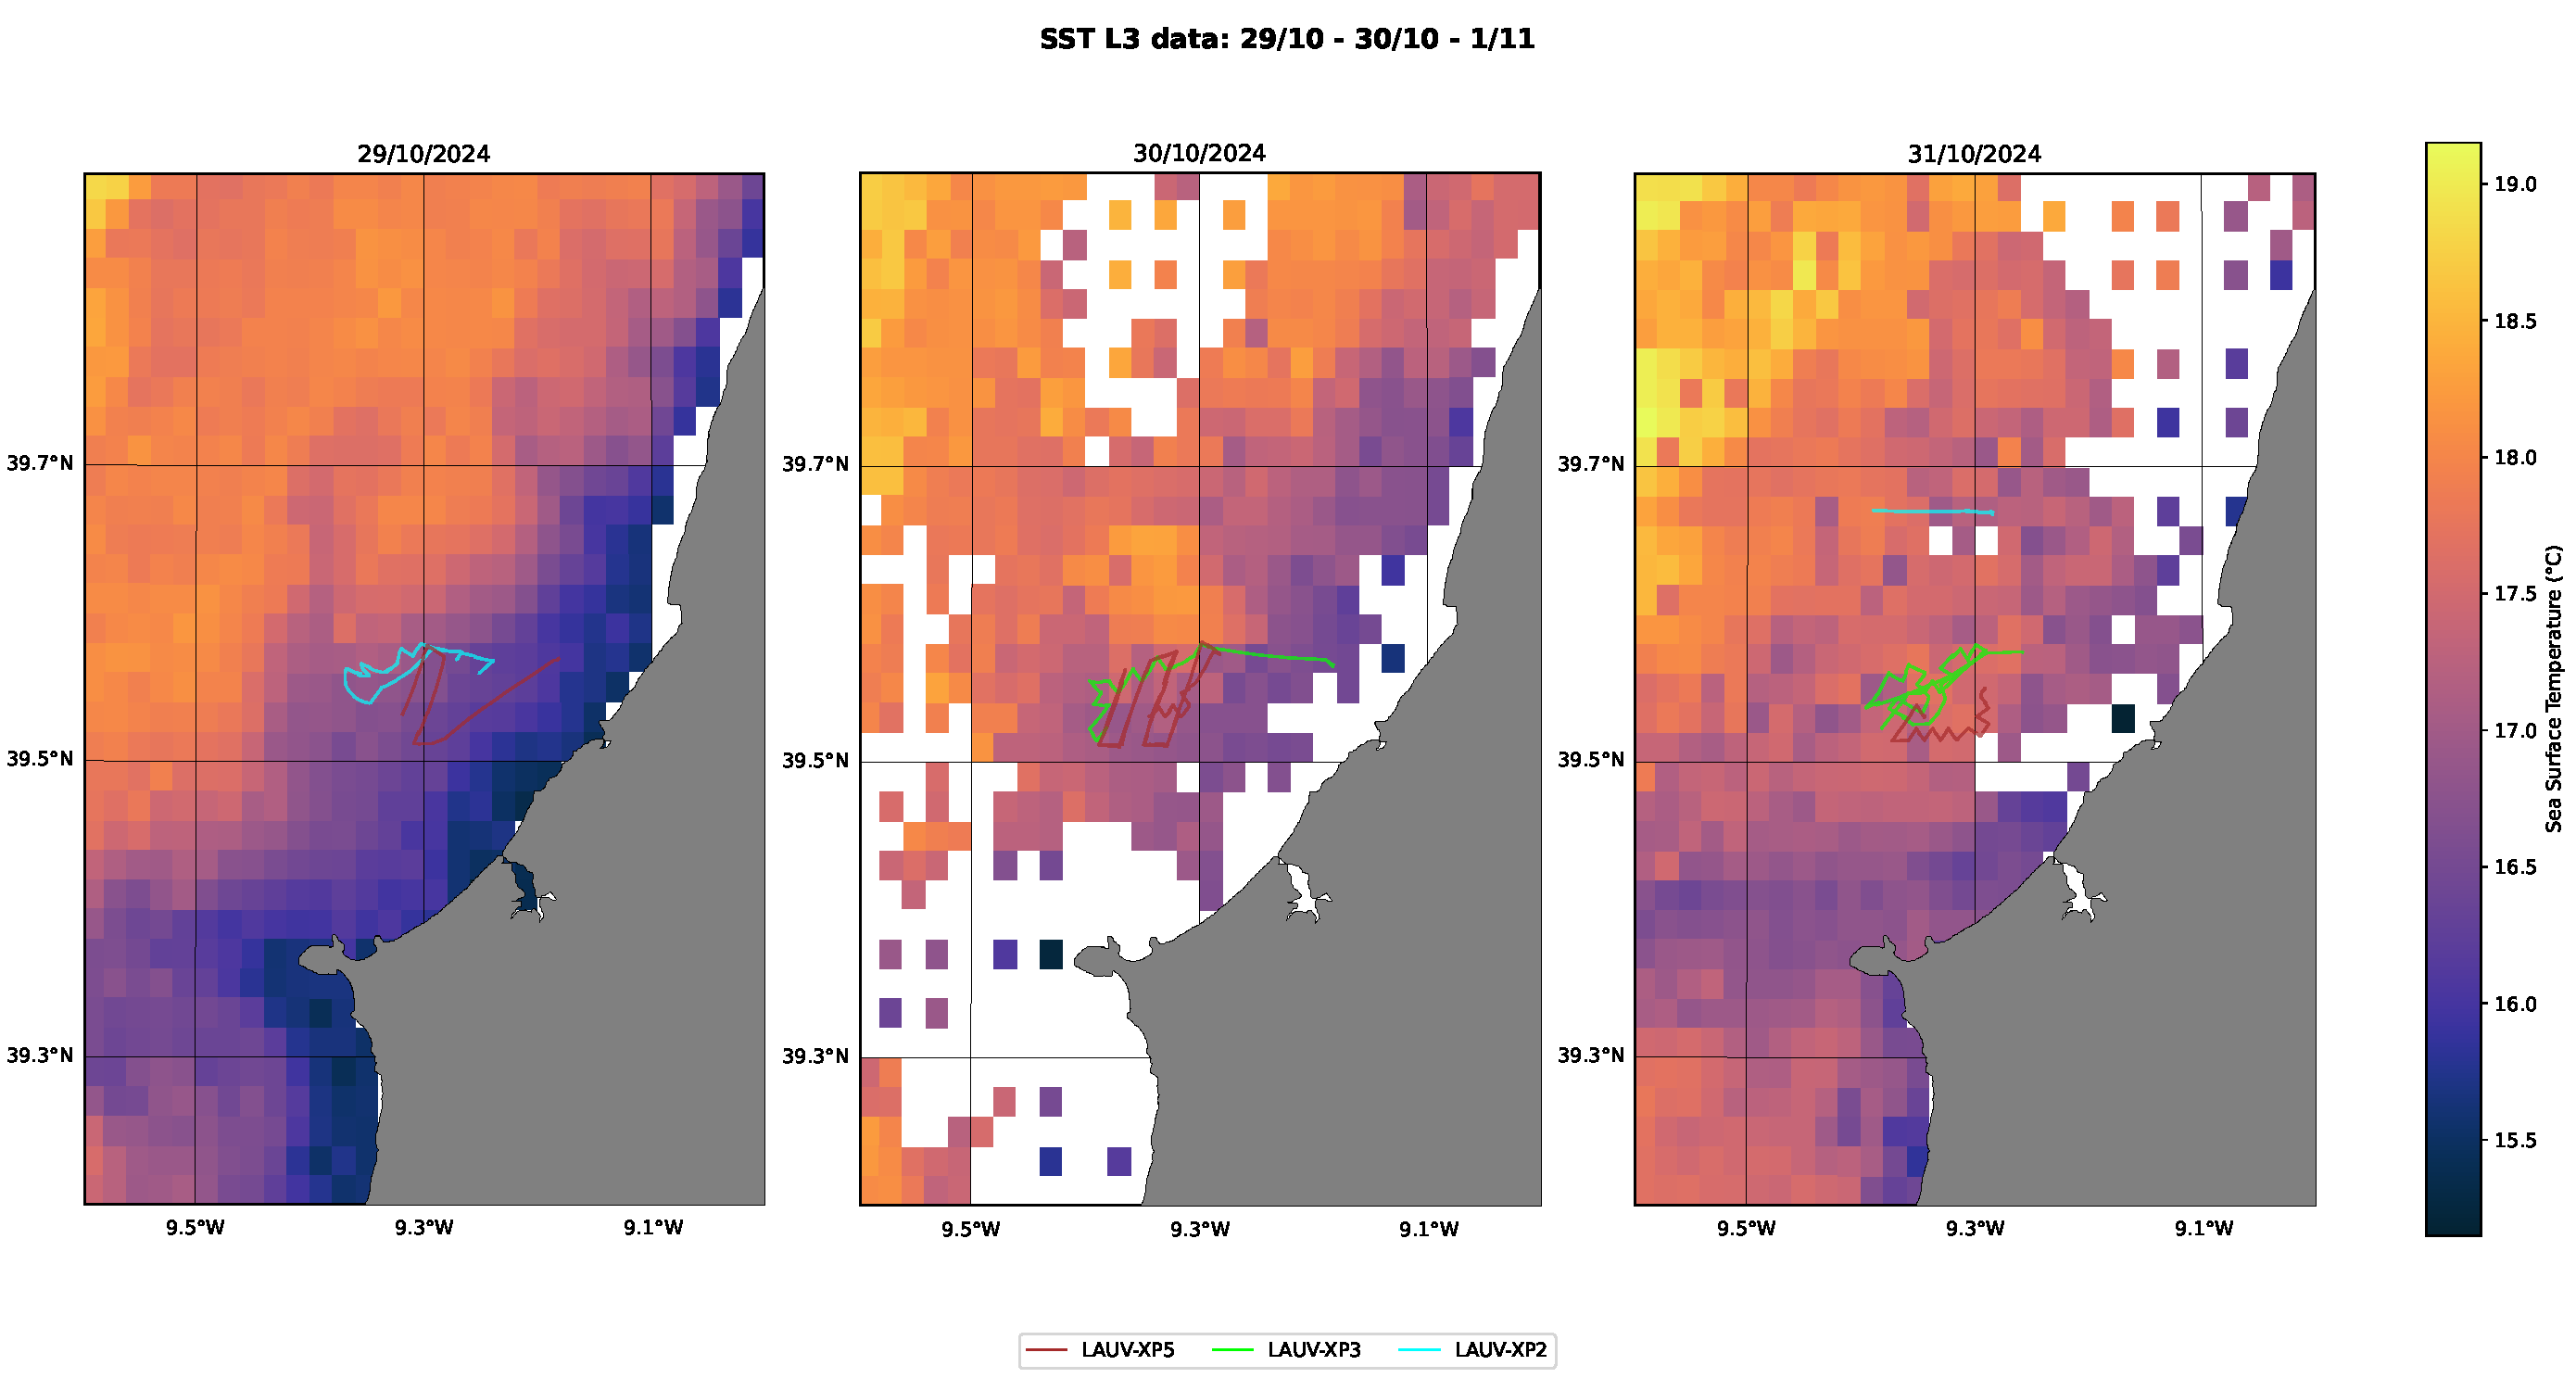
\includegraphics[width=1\linewidth]{fig/SST_L3_color1.pdf}
    \caption{L3 SST data + AUV trajectories over 3 days}
    \label{fig:temperatureprofiles}
\end{figure}

\begin{figure}
    \centering
    \includegraphics[width=1\linewidth]{fig/Figure2_100m.pdf}
    \caption{temperature data collected by AUV in depth (yy) over time (xx)}
    \label{fig:temperatureprofiles}
\end{figure}
    
    
    \item RMS table (all cases) + rms figure (just A+D cases)
\end{itemize}

 
\textit{- Use \textbf{subheadings} to organize different experiments or analyses.}
